\documentclass[8pt]{beamer}

% unverzichtbare Mathe-Befehle
\usepackage{amsmath}
% viele Mathe-Symbole
\usepackage{amssymb}
% Erweiterungen für amsmath
\usepackage{mathtools}

% Fonteinstellungen
\usepackage{fontspec}
% Latin Modern Fonts werden automatisch geladen

% deutsche Spracheinstellungen
\usepackage[ngerman]{babel}
%BUG in Biblatex wird hiermit gefixt
\providetoggle{blx@lang@captions@english}

\usepackage[
  math-style=ISO,    % ┐
  bold-style=ISO,    % │
  sans-style=italic, % │ ISO-Standard folgen
  nabla=upright,     % │
  partial=upright,   % ┘
  warnings-off={           % ┐
    mathtools-colon,       % │ unnötige Warnungen ausschalten
    mathtools-overbracket, % │
  },                       % ┘
]{unicode-math}

% traditionelle Fonts für Mathematik
\setmathfont{Latin Modern Math}
\setmathfont{XITS Math}[range={scr, bfscr}]
\setmathfont{XITS Math}[range={cal, bfcal}, StylisticSet=1]

% Zahlen und Einheiten
\usepackage[
  locale=DE,                   % deutsche Einstellungen
  separate-uncertainty=true,   % immer Fehler mit \pm
  per-mode=symbol-or-fraction, % / in inline math, fraction in display math
]{siunitx}

% richtige Anführungszeichen
\usepackage[autostyle]{csquotes}

% schöne Brüche im Text
\usepackage{xfrac}

% Grafiken können eingebunden werden
\usepackage{graphicx}

% Grafiken können in LaTex gemalt werden
\usepackage{tikz, pgfplots}

% Ermöglicht relative Positionierung von tikz-Nodes
\usetikzlibrary{positioning}

% Für Feynman-Graphen mit Tikz
\usepackage{feynmp-auto}

% Für komplexere Captions
\usepackage{caption}

\usepackage{tikz}

% Literaturverzeichnis
\usepackage[
  backend=biber,
  style=authoryear,
  autocite=inline,
]{biblatex}
% Quellendatenbank
\addbibresource{presentation.bib}

\usetheme[numbering=fraction]{metropolis}

% Für die Titelseite
%\title{The Influence of Music Genres on Performance Metrics: A Comparative Analysis of Spotify and YouTube}
\title{The Genre Factor}
\subtitle{Project Presentation - ML Seminar 2023}
\author{Henry Krämerkämper\\%
  \and%
  Christopher Breitfeld}
\institute{Technische Universität Dortmund}
\date{13.07.2023}
\logo{
\includegraphics[height=0.5cm]{figures/tu_logo_sw_klein.pdf}}

\begin{document}

\begin{frame}
  \titlepage
\end{frame}

\begin{frame}{Description of the Data Set}
    \begin{alertblock}{Dataset from \href{https://www.kaggle.com/datasets/salvatorerastelli/spotify-and-youtube}{Kaggle}: Spotify and YouTube}
      \begin{itemize}
        \item Contains statistics of songs on Spotify and YouTube
        \item $\SI{20.7}{\kilo}$ entries by $\SI{2}{\kilo}$ artists
        \item Does \alert{NOT} include the genre
      \end{itemize}
    \end{alertblock}
    \begin{alertblock}{Wikidata Query for the Top-Genre of the Artist}
      \begin{itemize}
       \item Query artist's Wikidata page for genre names
       \item Assign artists/album genre to song
      \end{itemize}
    \end{alertblock}
    \begin{columns}[T]
        \begin{column}{0.4\textwidth}
            \begin{alertblock}{Selection}
                \begin{itemize}
                    \item Groupe Subgenres into Overcategories
                    \item Select sample of $\num{6}$ Genres
                    \item Remaining Songs: $\num{6446}$
                \end{itemize}
            \end{alertblock}
        \end{column}
        \begin{column}{0.6\textwidth}
            \begin{figure}
                \hspace*{-1.7cm}
                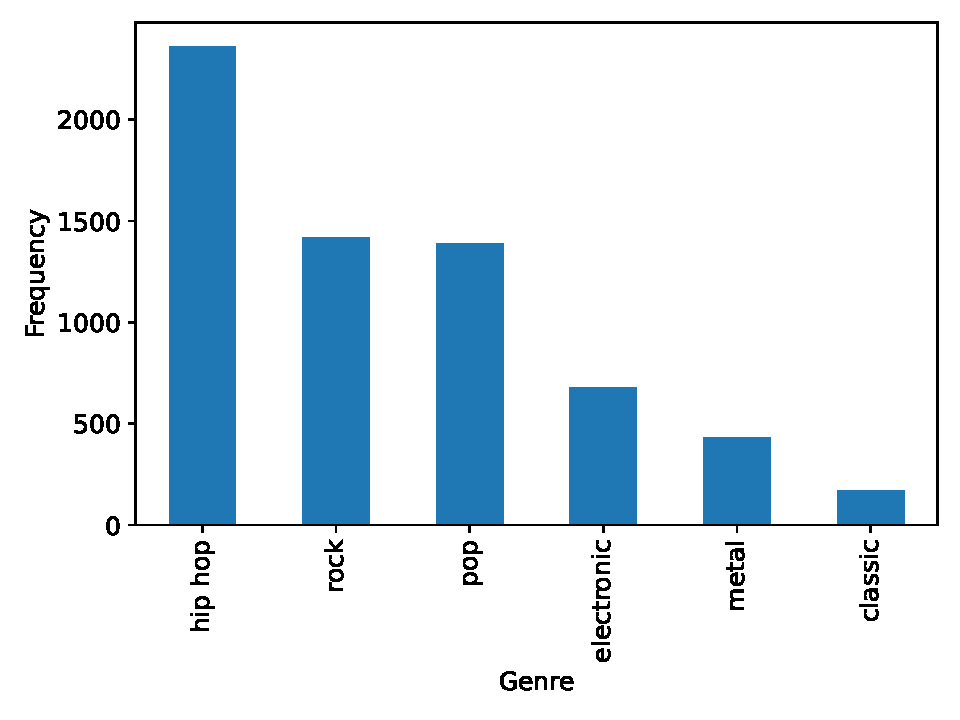
\includegraphics[width=1.1\textwidth]{../figures/genre_hist.pdf}
            \end{figure}
        \end{column}
    \end{columns}
\end{frame}
\begin{frame}
    \frametitle{Network Architecture}
    
    \begin{columns}[T]
        \begin{column}{0.4\textwidth}
            \begin{alertblock}{Model}
                \begin{itemize}
                    \item $\num{4}$ Dense Layers with Dropout
                    \item Loss function: categorical crossentropy
                    \item Optimizer: adam
                \end{itemize}    
            \end{alertblock}
        \end{column}
        \begin{column}{0.6\textwidth}
            \begin{figure}
                \hspace*{-1.7cm}
                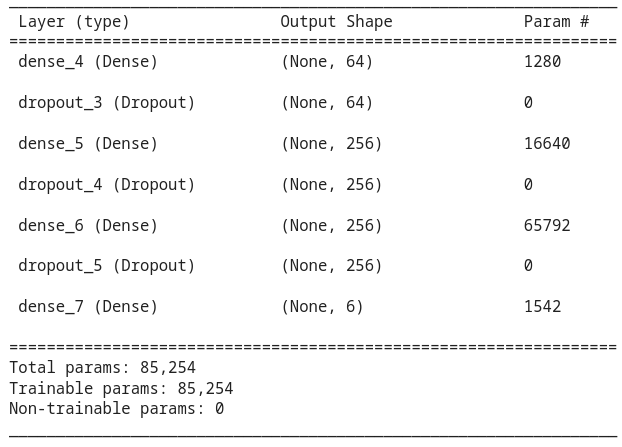
\includegraphics[width=1\textwidth]{../figures/model_summary.png}
            \end{figure}
        \end{column}
    \end{columns}

    \begin{alertblock}{Training}
        \begin{itemize}
            \item Early stopping: Stops training when the validation loss function no longer improves
            \item Reduce learning rate: Decreases learning rate if validation loss function stagnates \\
            \to better convergence
            \item Train the model using the training data with the defined set of hyperparameters.
        \end{itemize}  
    \end{alertblock}
    
\end{frame}
    
\begin{frame}
    \frametitle{Hyperparameter Optimization}
    
    \begin{alertblock}{Method}
        \begin{itemize}
            \item Grid Search
            \item Train models with all combinations of hyperparameters
        \end{itemize}    
    \end{alertblock}

    \begin{alertblock}{Validation}
        \begin{itemize}
            \item $k=\num{3}$ Cross Validation
            \item save train/validation Accuracy and Loss
        \end{itemize}
    \end{alertblock}

    \begin{figure}
        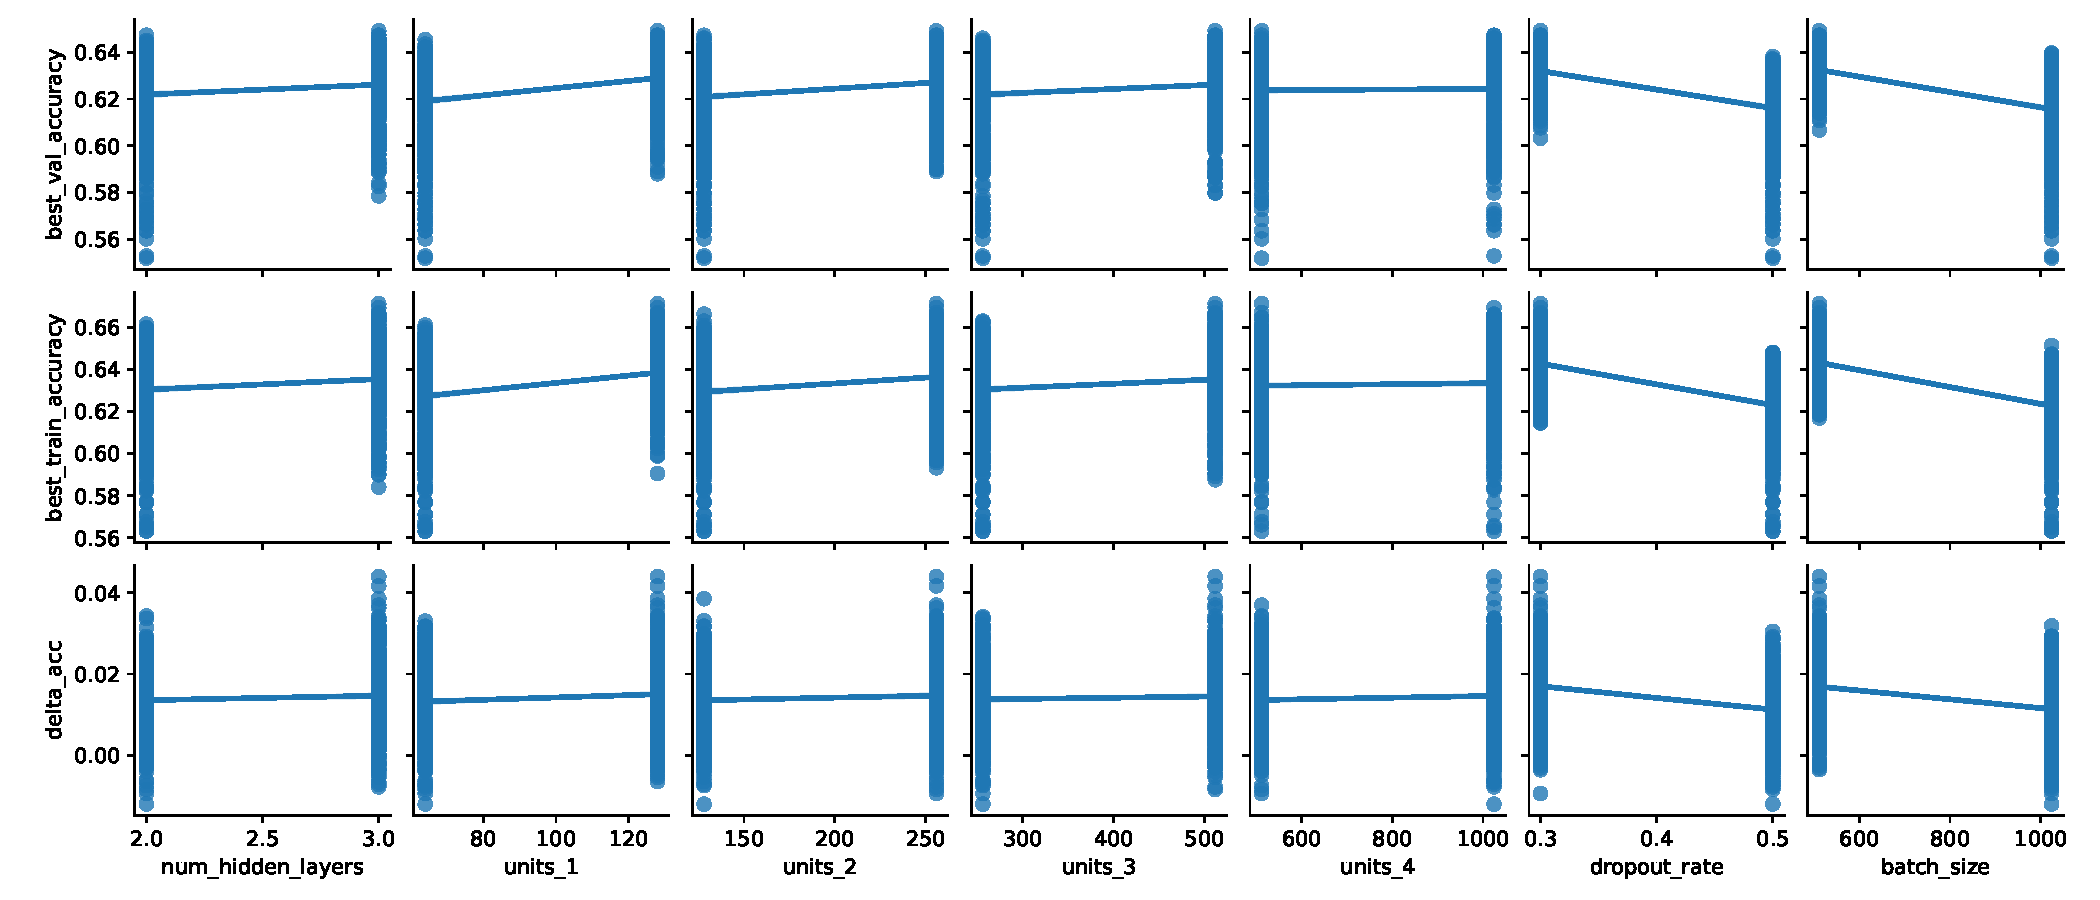
\includegraphics[scale=0.3]{../figures/HPO_parameter.pdf}
    \end{figure}

\end{frame}
\begin{frame}
    \frametitle{Overtraining Checks}
    
    \begin{alertblock}{Methods to prevent Overtraining}
        \begin{itemize}
            \item Dropout
            \item Early stopping
            \item minimize (Training Acc. - Validation Acc.) 
            \alert{but} maximize Validation Acc.
        \end{itemize}
    Try different values and decide after Hyperparameter Optimization
    \end{alertblock}
    \begin{figure}
        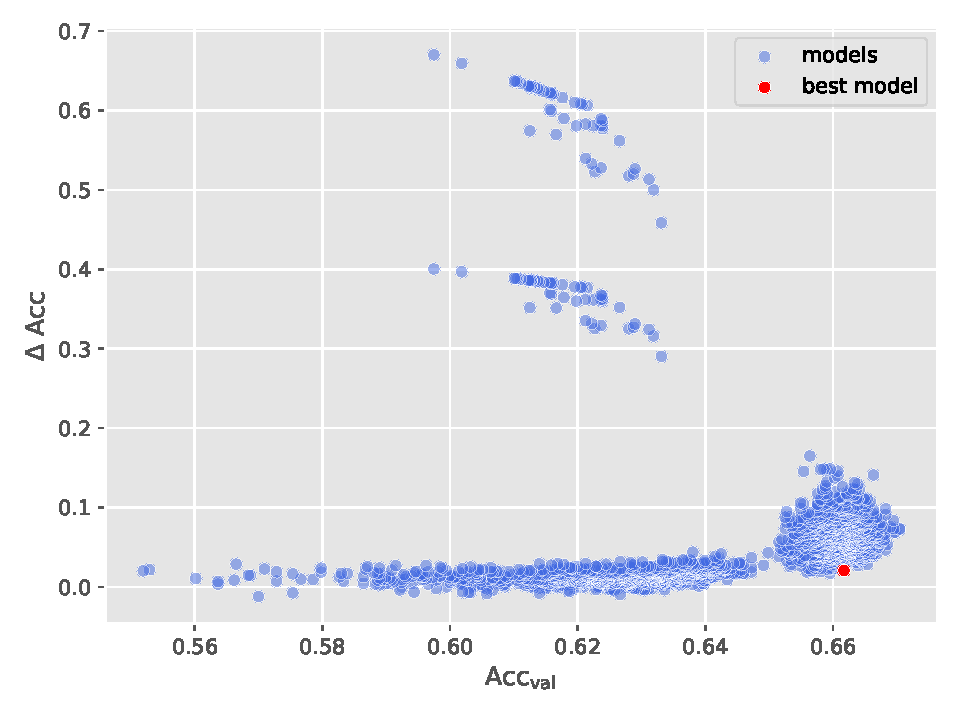
\includegraphics[scale=0.45]{../figures/HPO_scatter.pdf}
    \end{figure}
    
\end{frame}


% Alle Quellen, die bisher nicht zitiert wurden
%\nocite{Theories_of_grbs}

\printbibliography

\appendix
\begin{frame}
    \frametitle{Appendix: Accuracy and Loss}
    \begin{figure}
        \begin{minipage}[b]{0.48\textwidth}
            \centering
            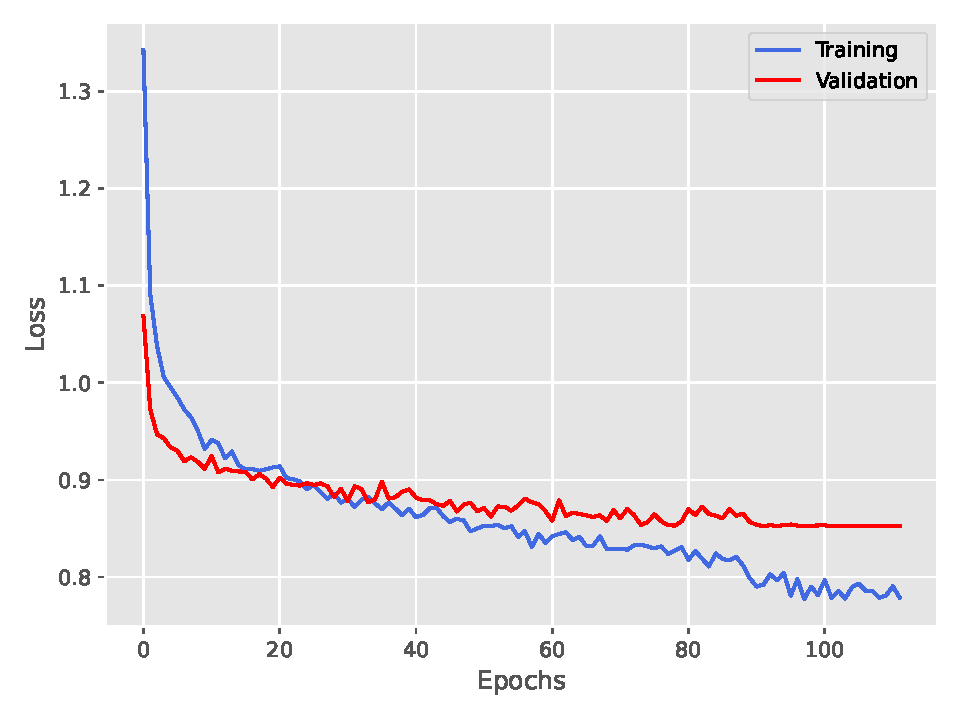
\includegraphics[width=\textwidth]{../figures/Loss.pdf}
        \end{minipage}
        \hfill
        \begin{minipage}[b]{0.48\textwidth}
            \centering
            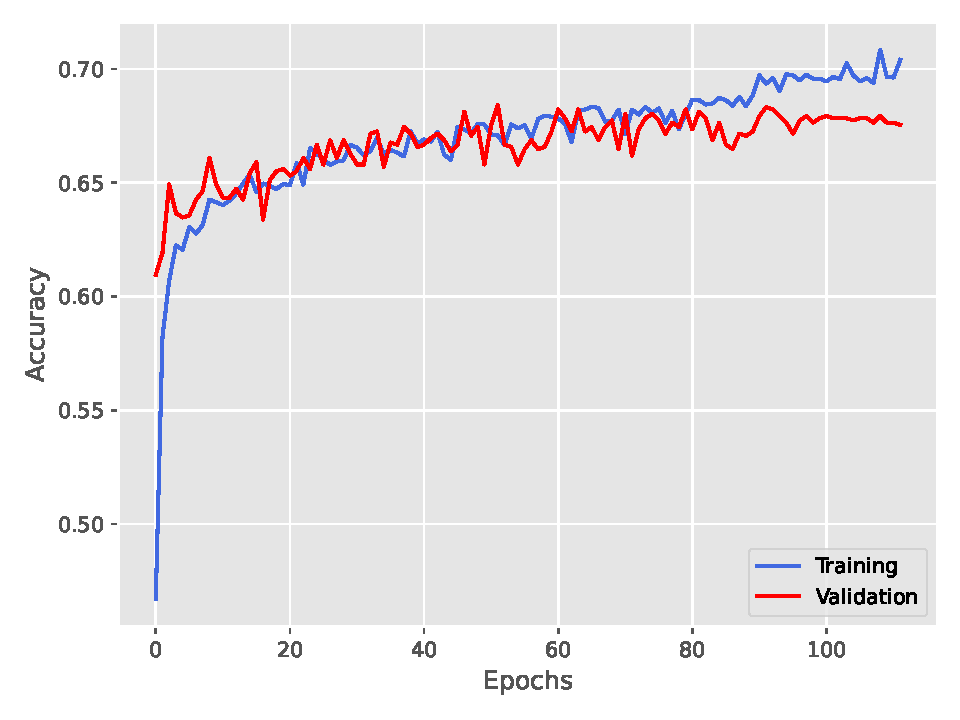
\includegraphics[width=\textwidth]{../figures/Acc.pdf}
        \end{minipage}
    \end{figure}
\end{frame}
\begin{frame}
    \frametitle{Appendix: Precision-Recall Curve}
    \begin{figure}
        \begin{minipage}[b]{0.48\textwidth}
            \centering
            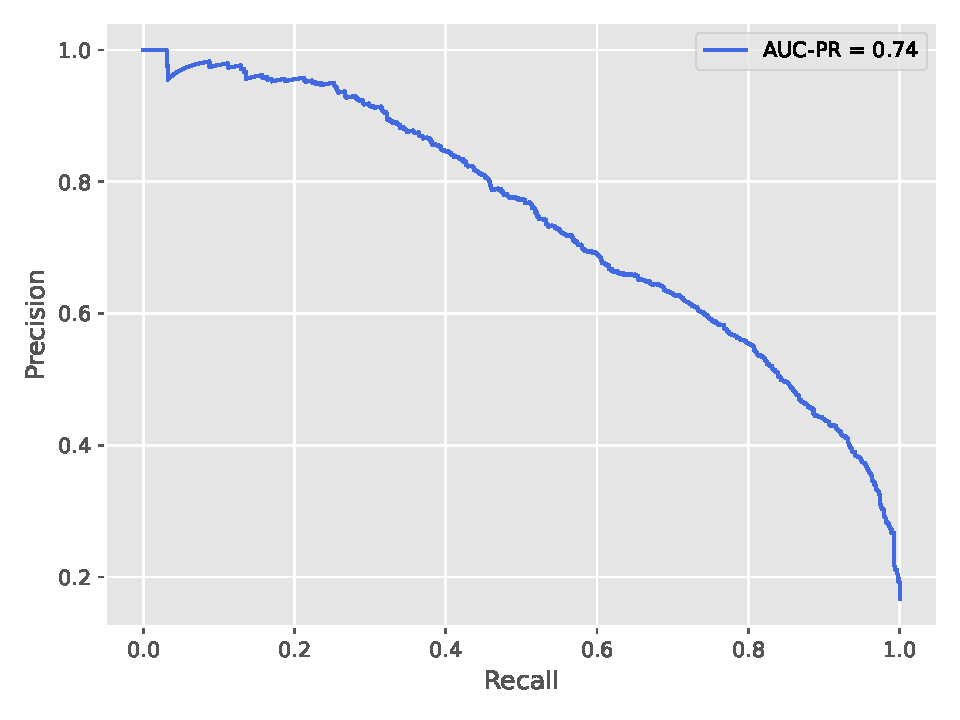
\includegraphics[width=\textwidth]{../figures/PR_curve.pdf}
        \end{minipage}
        \hfill
        \begin{minipage}[b]{0.48\textwidth}
            \centering
            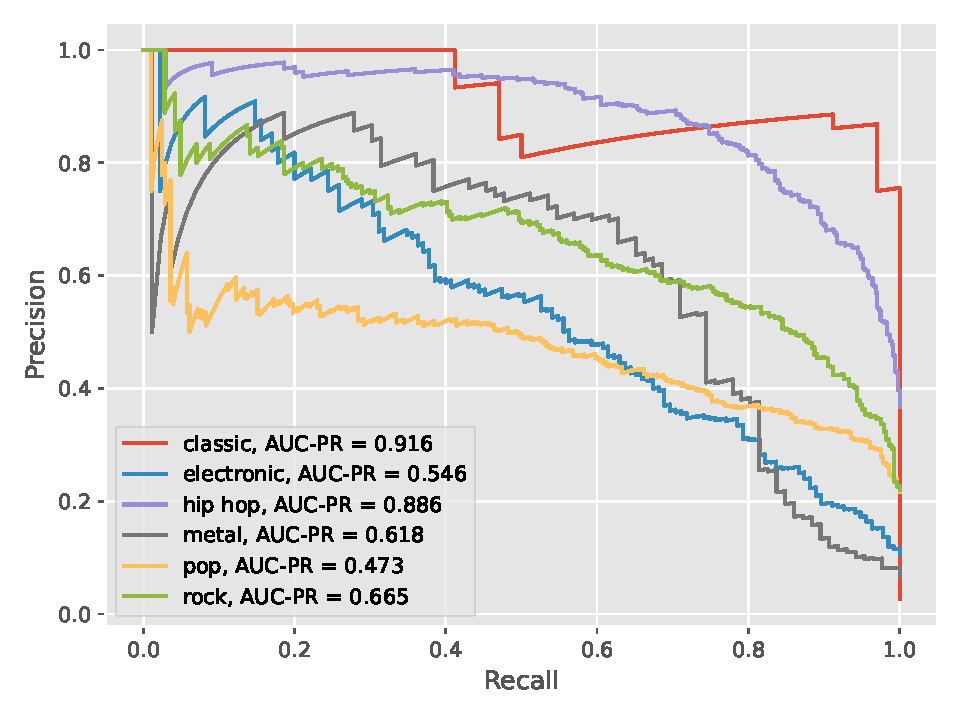
\includegraphics[width=\textwidth]{../figures/PR_curve_genres.pdf}
        \end{minipage}
    \end{figure}
\end{frame}
\begin{frame}
    \frametitle{Appendix: Substructure of Hip Hop}
    \begin{figure}
        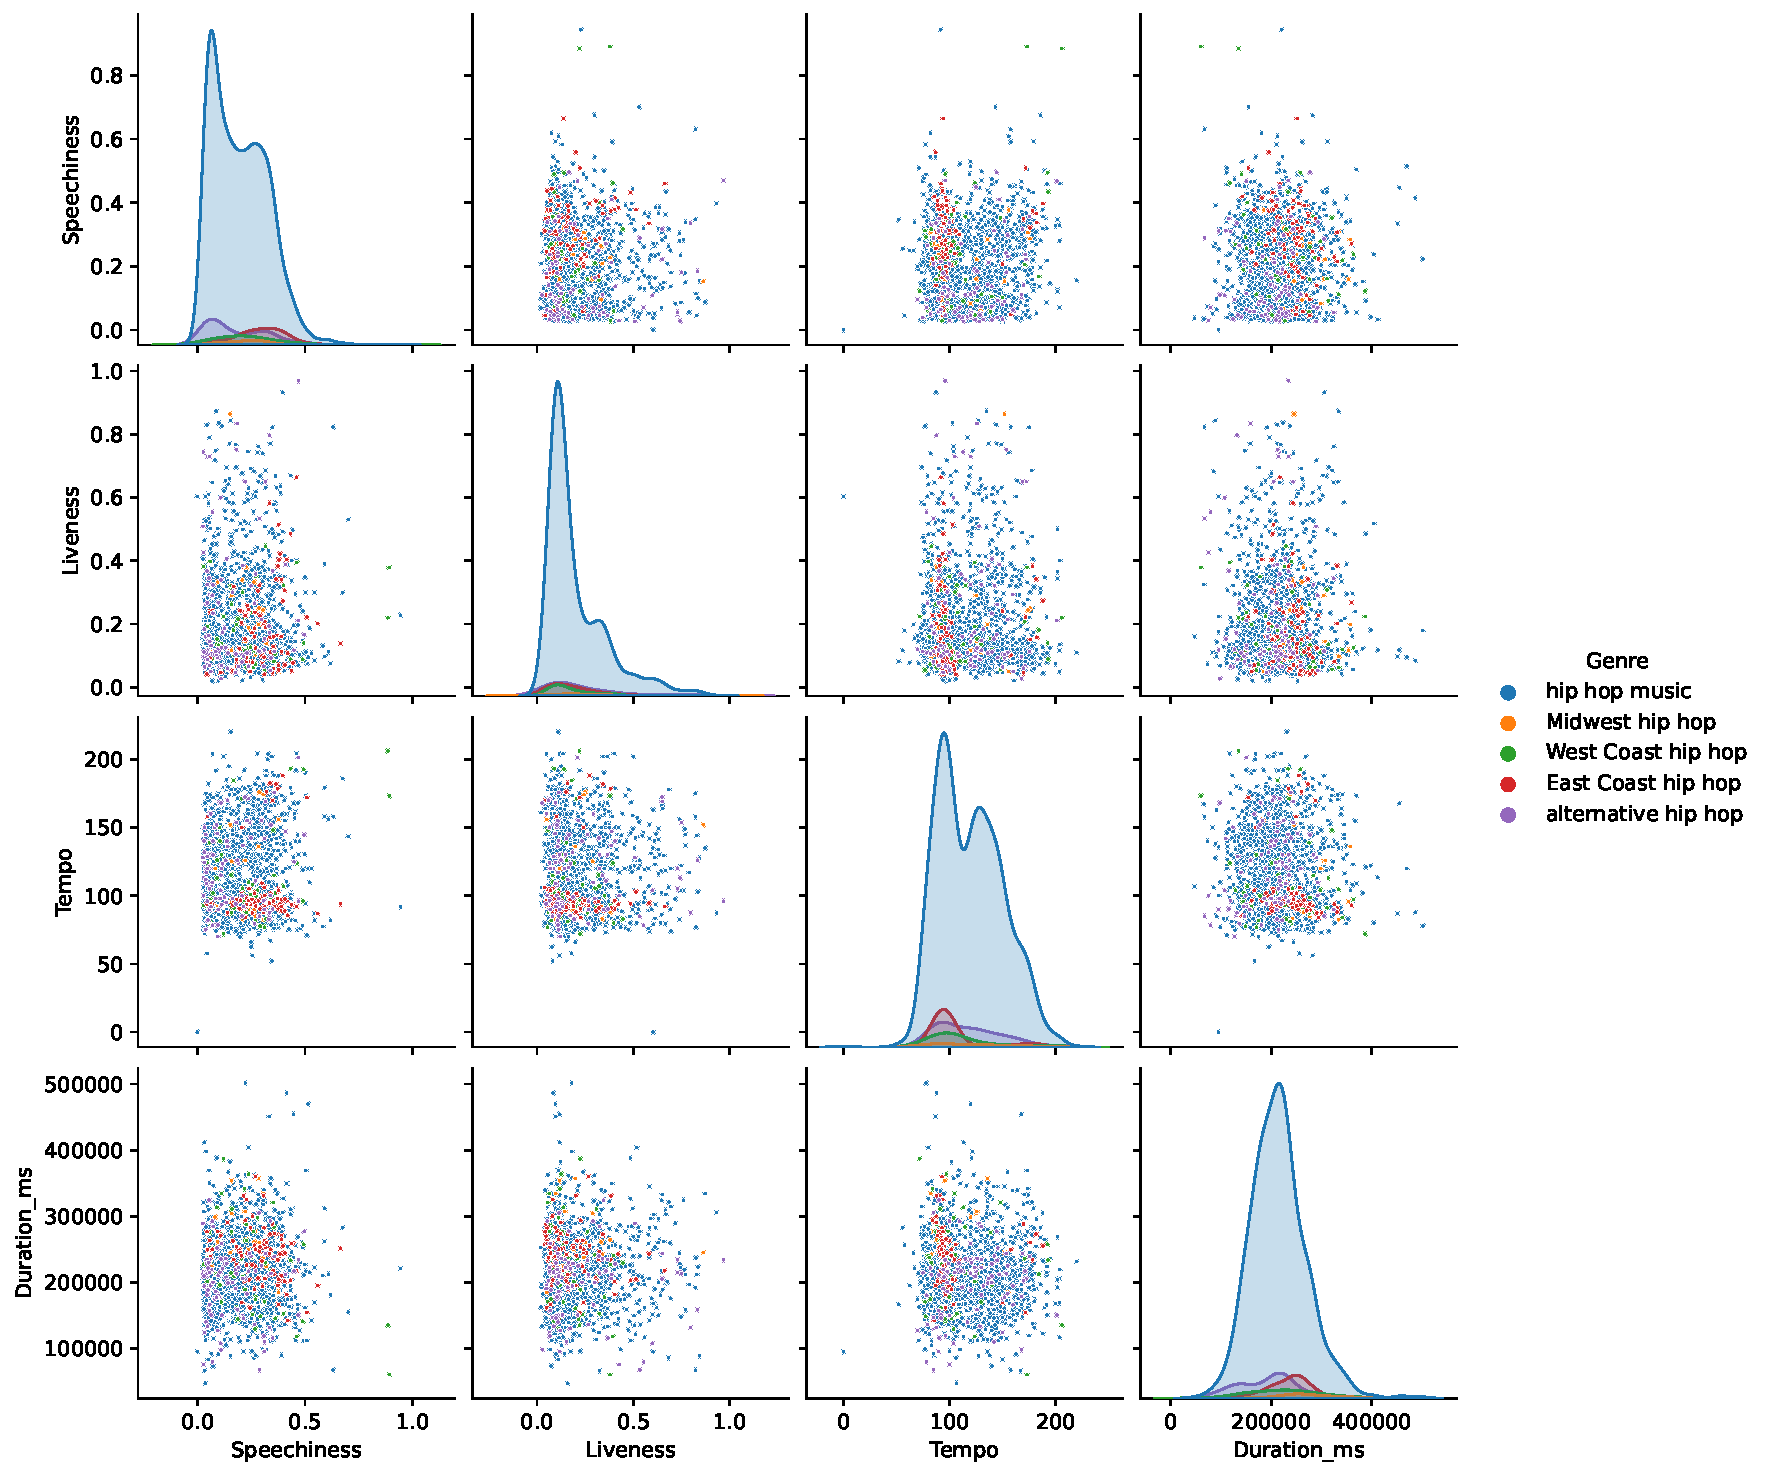
\includegraphics[scale=0.3]{../figures/pairplots/pairplot_hip_v3.pdf}
    \end{figure}
\end{frame}

\end{document}
